%%%%%%%%%%%%%%%%%%%%%%%%%%%%%%%%%%%%%%%%%%%%%%%%%%%%%%%%%%%%%%%
% P1 Thyroid
% David Miguel Lozano
% Javier Martínez Riberas
% Universidad de Burgos - Septiembre 2016
%%%%%%%%%%%%%%%%%%%%%%%%%%%%%%%%%%%%%%%%%%%%%%%%%%%%%%%%%%%%%%%

% -------------------------------------------------------------
% Preamble
% -------------------------------------------------------------
\documentclass[a4paper,12pt,titlepage]{article}

% -------------------------------------------------------------
% Packages
% -------------------------------------------------------------
\usepackage[utf8]{inputenc}	% Unicode support
\usepackage[T1]{fontenc}		% Font encoding
\usepackage[spanish]{babel}	% Languaje
\usepackage{lmodern}	% Typeface 
\usepackage{textcomp} % Special symbols
\usepackage{graphicx}	% Add pictures
\usepackage{pgfplots} % Graphs and charts
\usepackage{hyperref}	% Add a link to index entries
\usepackage{amsmath}	% Advanced math typesetting
\usepackage{amsfonts}	% Mathematical formulas
\usepackage{amssymb}	% Extended symbol collection
\usepackage{listings}	% Code formatting and highlighting
\usepackage{xcolor}		% Color package
\usepackage{enumitem}	% Customizing lists
\usepackage{parskip}	% Paragraph styles
\usepackage[a4paper]{geometry} 		% Margins
\usepackage[numbers,sort]{natbib}	% Bibliography management 

% -------------------------------------------------------------
% Configuration
% -------------------------------------------------------------
% Images path
\graphicspath{ {img/} }
% Graphs configuration 
\pgfplotsset{width=\textwidth,compat=1.9}
% Hyperlinks coloring
\hypersetup{
	colorlinks,
	linkcolor={green!40!black},
	citecolor={blue!50!black},
	urlcolor={blue!80!black}
}
% Define HRule
\newcommand{\HRule}[1]{\rule{\linewidth}{#1}}

\begin{document}
% -------------------------------------------------------------
% Cover
% -------------------------------------------------------------
\author{David Miguel Lozano \ Javier Martínez Riberas}
\title{P1 Thyroid}
\date{23-09-2016}

\begin{titlepage}
	\centering
	
\includegraphics[width=0.16\textwidth]{ubu-logo.png}\par
	\vspace{0.3cm}
	{\scshape\LARGE Universidad de Burgos \par}
	\vfill
	{\scshape\Large Computación Neuronal y Evolutiva \par}
	\HRule{2pt}
	{\huge\bfseries P1: Thyroid \par}
	\HRule{2pt}
	\\ [0.5cm]
	{Diseñar y entrenar una red neuronal para clasificar pacientes en tres grupos clínicos dependiendo de la patología en la glándula tiroides (pacientes sanos, con hipertiroidismo o con hipertiroidismo).}
	\vfill
	Estudiantes:\par
	{\Large\scshape David Miguel Lozano \\ Javier Martínez Riberas \par}
	\vfill
	Profesor de la asignatura:\par
	\textsc{Álvaro Herrero Cosío}
	\vfill
	{\large 1º semestre 2016 \par}
\end{titlepage}

% -------------------------------------------------------------
% Contents
% -------------------------------------------------------------
\newpage
\tableofcontents
\begin{appendix}
  %\listoffigures
  %\listoftables
\end{appendix}

% -------------------------------------------------------------
% Body
% -------------------------------------------------------------
\newpage

\section{Introduction}

El objetivo de la práctica es diseñar y entrenar una red neuronal para la clasificación de pacientes en tres grupos dependiendo de la patología en la glándula tiroides. Se trata de un problema de reconocimiento de patrones en el que dados unos datos de entrada, la red neuronal será capaz de asignarlos a una de las tres clases definidas (pacientes sanos, con hipertiroidismo o con hipotiroidismo). Haremos uso del dataset de ejemplo \emph{Thyroid} que provee Matlab.

Realizaremos un estudio sobre el ajuste en el número de neuronas, ejecutando varios entrenamientos con la red y modificando el valor de este parámetro. También estudiaremos el rendimiento que proporcionan los diferentes algoritmos de entrenamiento  incluidos en Matlab. Por último, discutiremos qué configuración nos proporciona los mejores resultados, explotaremos la red y analizaremos las salidas devueltas.

\section{Motivación}

La motivación que nos llevó a elegir el tema del trabajo fue el que ambos poseíamos algún familiar que sufría alguna alteración en la glándula tiroides. Además, el gran desarrollo que están teniendo las redes neuronales aplicadas a la medicina en los últimos años (ej. IBM Watson \citep{wiki:watson}) nos desató interés para adentrarnos en este tema.

\section{Descripción del conjunto de datos}

El conjunto de datos utilizados los hemos obtenido del dataset de ejemplo \emph{Thyroid} que provee Matlab. Los datos provienen del \emph{UCI Machine Learning Repository} \citep{Asuncion+Newman:2007} y fueron donados por la Universidad de California.

El dataset contiene datos de 7200 pacientes agrupados en dos matrices:

\begin{itemize}[noitemsep]
	\item $thyroidInputs$: matriz de 21x7200 con los datos de los 7200 pacientes caracterizados por 15 atributos binarios y 6 atributos continuos.
	\item $thyroidTargets$: matriz de 3x7200 en donde se asocia un vector de tres clases a cada paciente. En este vector se define a cuál de las tres clases pertenece el paciente.
\end{itemize}

\newpage

Las tres clases que contiene el dataset son:

\begin{enumerate}[noitemsep]
	\item Paciente sano.
	\item Paciente con hipertiroidismo.
	\item Paciente con hipotiroidismo.
\end{enumerate}

La descripción precisa del significado real de cada atributo y los valores que puede tomar la podemos encontrar en la página web del repositorio \citep{Asuncion+Newman:2007}. Para nuestra tarea no nos es relevante.

Nuestro objetivo es construir una red neuronal y entrenarla con los datos reales proporcionados para que posteriormente sea capaz de clasificar a nuevos pacientes. 

Dividiremos aleatoriamente los datos que contiene el data set en tres grupos:

\begin{itemize}[noitemsep]
	\item $Training (70\%)$: lo utilizaremos para el entrenamiento supervisado.
	\item $Validation (15\%)$: lo utilizaremos para comprobar cuándo la red está generalizando y detener el entrenamiento para evitar el sobreajuste (\textit{overfitting}).
	\item $Test (15\%)$: lo utilizaremos de forma totalmente independiente al entrenamiento para comprobar la generalización de la red.
\end{itemize}

\section{Descripción del procedimiento}

Para resolver la tarea planteada creamos una red neuronal con una topología \href{http://www.mathworks.com/help/nnet/ref/patternnet.html}{patternnet}. Esta topología posee dos capas \textit{feedforward}, con una función de activación sigmoidal en la capa oculta y una función \textit{softmax} en la capa de salida. Se caracteriza por poder clasificar vectores con una precisión arbitrariamente buena si posee suficientes neuronas en su capa oculta.

\begin{figure}[!ht]
	\centering
	\label{fig:patternnet}
	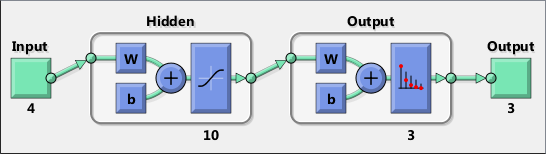
\includegraphics[width=\textwidth]{patternnet.png}
	\caption{Pattern recognition network.}
\end{figure}

En nuestro estudio vamos a variar el número de neuronas de la capa oculta para intentar conseguir los mejores resultados (tanto en error, como en tiempo de entrenamiento). La capa de salida siempre va a tener tres neuronas, cada una se encargará de evaluar la pertenencia a una de las tres clases.

Otro elemento que puede afectar al rendimiento de nuestra red es la función de entrenamiento utilizada. Probaremos ocho funciones distintas que implementa Matlab para comparar resultados.

Para realizar el estudio lo más automatizado posible, hemos creado una función ($autoTrain$) que se encarga de entrenar la red de acuerdo con los parámetros pasados. Por otro lado tenemos un script ($trainAndShow.m$) que llama a esta función variando el número de neuronas de la capa oculta (de 1 a 50 con paso 1) y los algoritmos de entrenamiento ($trainbfg$, $trainrp$, $trainscg$, $traincgb$,  $traincgf$, $traincgp$, $trainoss$ y $traingdx$). Además, repite el entrenamiento de cada caso 10 veces para disminuir la varianza y la aleatoriedad.

El script proporciona como salida el valor de confusión medio en cada caso,  la matriz de confusión completa y el tiempo medio de entrenamiento. Con tres formatos de salida, un primer formato legible para humanos, otro formateado para la librería de gráficos \textit{pgfplots} y un tercer formato como CSV.

\emph{*Todo el código generado en esta práctica se encuentra disponible en el siguiente repositorio: 
\href{https://github.com/davidmigloz/neuronal-networks/tree/master/P1\_Thyroid}{P1\_Thyroid}.}

\section{Estudio}

Tras realizar la ejecución del programa descrito en la sección anterior, hemos obtenido los datos que se muestran en las siguientes gráficas.

En las dos primeras se muestra, para cada algoritmo de entrenamiento, la evolución del valor de confusión total ponderado de todos los conjuntos de datos (entrenamiento, validación y pruebas) según se incrementa el número de neuronas en la capa oculta. 

\textit{*Hemos dividido los resultados en dos gráficas para mejorar la legibilidad de las mismas.}

En las dos segundas se muestra la evolución del tiempo empleado en el entrenamiento de la red neuronal según se aumenta el número de neuronas en la capa oculta.

\newpage
\newgeometry{top=1cm,bottom=2.5cm}

\begin{tikzpicture}[every plot/.append style={semithick}]
\begin{axis}[
    title={Evolución del valor de confusión},
    xlabel={Número de neuronas en la capa oculta},
    ylabel={Valor de confusión},
    xmin=1, xmax=50,
    ymin=0.03, ymax=0.08,
    xtick={1,10,20,30,40,50},
    ytick={0.03,0.04,0.05,0.06,0.07,0.08},
    legend pos=north east,
    ymajorgrids=true,
    grid style=dashed,
    scaled ticks=false, % prevent scale labels
    tick label style={/pgf/number format/fixed}, % label number format
]

\addplot
    coordinates {
(1,0.074167)(2,0.067764)(3,0.072556)(4,0.059986)(5,0.057514)(6,0.062403)(7,0.056681)(8,0.047250)(9,0.051042)(10,0.052542)(11,0.045278)(12,0.054181)(13,0.053569)(14,0.042542)(15,0.055014)(16,0.049542)(17,0.055556)(18,0.052361)(19,0.053528)(20,0.048111)(21,0.051292)(22,0.045903)(23,0.050306)(24,0.050194)(25,0.053056)(26,0.046681)(27,0.053514)(28,0.051917)(29,0.055444)(30,0.048000)(31,0.051528)(32,0.058431)(33,0.053972)(34,0.050458)(35,0.047583)(36,0.047458)(37,0.047056)(38,0.056722)(39,0.053889)(40,0.056097)(41,0.049056)(42,0.041597)(43,0.056153)(44,0.039375)(45,0.050208)(46,0.046194)(47,0.041042)(48,0.050111)(49,0.052472)(50,0.050347)
    };
    \addlegendentry{trainbfg}
    
\addplot
    coordinates {
(1,0.074181)(2,0.070847)(3,0.063333)(4,0.060000)(5,0.056931)(6,0.056750)(7,0.057264)(8,0.055611)(9,0.056000)(10,0.056083)(11,0.056458)(12,0.056667)(13,0.056736)(14,0.057472)(15,0.055014)(16,0.057139)(17,0.057514)(18,0.057986)(19,0.056403)(20,0.054583)(21,0.057986)(22,0.056278)(23,0.054333)(24,0.055347)(25,0.055389)(26,0.055708)(27,0.053361)(28,0.056000)(29,0.054486)(30,0.054806)(31,0.056333)(32,0.054403)(33,0.053264)(34,0.054028)(35,0.055625)(36,0.053056)(37,0.052972)(38,0.054472)(39,0.055292)(40,0.055917)(41,0.057125)(42,0.056583)(43,0.056417)(44,0.055194)(45,0.055458)(46,0.054111)(47,0.053250)(48,0.056083)(49,0.054125)(50,0.055806)
    };
    \addlegendentry{trainrp}

\addplot
    coordinates {
(1,0.063875)(2,0.065778)(3,0.058097)(4,0.060972)(5,0.059389)(6,0.057083)(7,0.054361)(8,0.056097)(9,0.056750)(10,0.055972)(11,0.057208)(12,0.056389)(13,0.057861)(14,0.055403)(15,0.059819)(16,0.056153)(17,0.058431)(18,0.056194)(19,0.057917)(20,0.055889)(21,0.056556)(22,0.057375)(23,0.054333)(24,0.054028)(25,0.059292)(26,0.054653)(27,0.055458)(28,0.056833)(29,0.056181)(30,0.057194)(31,0.056403)(32,0.057361)(33,0.055264)(34,0.055569)(35,0.059319)(36,0.057319)(37,0.055694)(38,0.055597)(39,0.054681)(40,0.055653)(41,0.053611)(42,0.056278)(43,0.056875)(44,0.056333)(45,0.056903)(46,0.056347)(47,0.058278)(48,0.056514)(49,0.059444)(50,0.058486)
    };
    \addlegendentry{trainscg}

\addplot
    coordinates {
(1,0.068264)(2,0.063472)(3,0.057083)(4,0.055625)(5,0.047528)(6,0.052111)(7,0.041444)(8,0.043597)(9,0.052389)(10,0.052708)(11,0.037736)(12,0.053139)(13,0.051111)(14,0.039222)(15,0.048972)(16,0.041750)(17,0.049681)(18,0.048569)(19,0.050389)(20,0.042944)(21,0.042167)(22,0.052944)(23,0.050875)(24,0.054625)(25,0.051889)(26,0.055792)(27,0.043736)(28,0.046569)(29,0.047069)(30,0.052639)(31,0.046028)(32,0.049569)(33,0.047792)(34,0.050792)(35,0.047417)(36,0.044194)(37,0.050417)(38,0.048458)(39,0.045444)(40,0.045958)(41,0.048083)(42,0.052958)(43,0.042139)(44,0.054986)(45,0.055375)(46,0.042139)(47,0.046931)(48,0.054139)(49,0.049958)(50,0.049264)
    };
    \addlegendentry{traincgb}
                    
\end{axis}
\end{tikzpicture}

\begin{tikzpicture}[every plot/.append style={semithick}]
\begin{axis}[
    xlabel={Número de neuronas en la capa oculta},
    ylabel={Valor de confusión},
    xmin=1, xmax=50,
    ymin=0.035, ymax=0.08,
    xtick={1,10,20,30,40,50},
    ytick={0.03,0.04,0.05,0.06,0.07,0.08},
    legend pos=south east,
    ymajorgrids=true,
    grid style=dashed,
    scaled ticks=false, % prevent scale labels
    tick label style={/pgf/number format/fixed}, % label number format
]

\addplot
    coordinates {
(1,0.074139)(2,0.072153)(3,0.072778)(4,0.069181)(5,0.067347)(6,0.065806)(7,0.064931)(8,0.061042)(9,0.057458)(10,0.063597)(11,0.056097)(12,0.059361)(13,0.061944)(14,0.057792)(15,0.059236)(16,0.057292)(17,0.053972)(18,0.053472)(19,0.058014)(20,0.053375)(21,0.052181)(22,0.054917)(23,0.052556)(24,0.051194)(25,0.050653)(26,0.055250)(27,0.055931)(28,0.055069)(29,0.051500)(30,0.056306)(31,0.051736)(32,0.053042)(33,0.052792)(34,0.052500)(35,0.048514)(36,0.051083)(37,0.054625)(38,0.050236)(39,0.044972)(40,0.050875)(41,0.053472)(42,0.053611)(43,0.045056)(44,0.048708)(45,0.050583)(46,0.044375)(47,0.047903)(48,0.049319)(49,0.051167)(50,0.051181)
    };
    \addlegendentry{traincgf}

\addplot
    coordinates {
(1,0.070389)(2,0.067708)(3,0.059181)(4,0.060194)(5,0.055764)(6,0.057319)(7,0.055597)(8,0.055903)(9,0.055014)(10,0.056458)(11,0.057292)(12,0.053292)(13,0.055042)(14,0.052236)(15,0.055306)(16,0.057292)(17,0.053208)(18,0.053736)(19,0.057653)(20,0.049958)(21,0.056917)(22,0.057708)(23,0.054375)(24,0.055125)(25,0.057097)(26,0.057014)(27,0.056083)(28,0.053764)(29,0.056694)(30,0.052292)(31,0.057222)(32,0.051361)(33,0.054917)(34,0.054111)(35,0.055319)(36,0.050361)(37,0.053625)(38,0.054431)(39,0.055361)(40,0.052903)(41,0.052972)(42,0.055028)(43,0.050861)(44,0.051958)(45,0.054861)(46,0.057944)(47,0.054361)(48,0.058597)(49,0.052514)(50,0.056875)
    };
    \addlegendentry{traincgp}
    
\addplot
    coordinates {
(1,0.070778)(2,0.067583)(3,0.067639)(4,0.057319)(5,0.062194)(6,0.057194)(7,0.064000)(8,0.057708)(9,0.054972)(10,0.059250)(11,0.054778)(12,0.057083)(13,0.056639)(14,0.058875)(15,0.056736)(16,0.055708)(17,0.054681)(18,0.054069)(19,0.057181)(20,0.056542)(21,0.057153)(22,0.053306)(23,0.056556)(24,0.058861)(25,0.057556)(26,0.056264)(27,0.057014)(28,0.057736)(29,0.056639)(30,0.056792)(31,0.057000)(32,0.056375)(33,0.057361)(34,0.057222)(35,0.055375)(36,0.057250)(37,0.058861)(38,0.056028)(39,0.055319)(40,0.053125)(41,0.055181)(42,0.056861)(43,0.056931)(44,0.055986)(45,0.055903)(46,0.057708)(47,0.056708)(48,0.057236)(49,0.056292)(50,0.057097)
    };
    \addlegendentry{trainoss}
    
\addplot
    coordinates {
(1,0.074167)(2,0.073556)(3,0.070833)(4,0.071528)(5,0.069014)(6,0.069917)(7,0.069903)(8,0.069375)(9,0.067472)(10,0.067264)(11,0.067181)(12,0.065806)(13,0.069958)(14,0.066528)(15,0.067736)(16,0.064764)(17,0.069250)(18,0.068111)(19,0.065111)(20,0.065056)(21,0.067000)(22,0.067611)(23,0.066250)(24,0.066000)(25,0.067931)(26,0.068875)(27,0.068139)(28,0.064514)(29,0.067931)(30,0.066625)(31,0.069069)(32,0.068611)(33,0.069319)(34,0.066792)(35,0.078778)(36,0.067764)(37,0.077833)(38,0.071222)(39,0.078681)(40,0.064389)(41,0.072486)(42,0.069694)(43,0.069694)(44,0.076792)(45,0.077736)(46,0.083389)(47,0.078472)(48,0.067000)(49,0.073889)(50,0.069681)
    };
    \addlegendentry{traingdx}      
                        
\end{axis}
\end{tikzpicture}

\newpage

\begin{tikzpicture}[every plot/.append style={semithick}]
\begin{axis}[
    title={Evolución del tiempo de entrenamiento},
    xlabel={Número de neuronas en la capa oculta},
    ylabel={Tiempo (s)},
    xmin=1, xmax=50,
    ymin=0, ymax=5,
    xtick={1,10,20,30,40,50},
    legend pos=north east,
    ymajorgrids=true,
    grid style=dashed,
    scaled ticks=false, % prevent scale labels
    tick label style={/pgf/number format/fixed}, % label number format
]

\addplot
    coordinates {
(1,0.801562)(2,0.773438)(3,0.879687)(4,1.398438)(5,2.479687)(6,1.701563)(7,2.498438)(8,3.678125)(9,4.343750)(10,4.023438)(11,5.843750)(12,5.215625)(13,5.926563)(14,8.187500)(15,6.839062)(16,9.581250)(17,9.698438)(18,11.779688)(19,11.412500)(20,14.092188)(21,13.120313)(22,20.200000)(23,18.621875)(24,21.139063)(25,19.675000)(26,23.539063)(27,20.375000)(28,25.926562)(29,24.084375)(30,32.139063)(31,27.175000)(32,23.542188)(33,26.528125)(34,35.023438)(35,42.085938)(36,47.539063)(37,48.171875)(38,40.892187)(39,50.700000)(40,53.690625)(41,69.996875)(42,86.618750)(43,60.521875)(44,129.239062)(45,90.700000)(46,129.045312)(47,143.954688)(48,126.051563)(49,121.410938)(50,127.959375)
    };
    \addlegendentry{trainbfg}
    
\addplot
    coordinates {
(1,0.329688)(2,0.351563)(3,0.628125)(4,0.592187)(5,0.707812)(6,0.778125)(7,0.700000)(8,0.676562)(9,0.767188)(10,0.748437)(11,0.825000)(12,0.803125)(13,0.814063)(14,0.703125)(15,0.890625)(16,0.831250)(17,0.756250)(18,0.700000)(19,0.901563)(20,0.984375)(21,0.746875)(22,0.828125)(23,1.146875)(24,0.912500)(25,0.971875)(26,0.950000)(27,1.126562)(28,0.851563)(29,1.015625)(30,1.064062)(31,0.967187)(32,1.065625)(33,1.168750)(34,1.160938)(35,1.134375)(36,1.087500)(37,1.125000)(38,1.139063)(39,0.984375)(40,1.028125)(41,0.910937)(42,0.946875)(43,1.007813)(44,1.143750)(45,1.193750)(46,1.290625)(47,1.482813)(48,1.103125)(49,1.267187)(50,1.156250)
    };
    \addlegendentry{trainrp}

\addplot
    coordinates {
(1,0.514062)(2,0.523438)(3,0.721875)(4,0.731250)(5,0.721875)(6,0.801562)(7,0.982812)(8,0.837500)(9,0.823438)(10,0.920312)(11,0.925000)(12,1.032812)(13,0.835938)(14,0.970313)(15,1.203125)(16,1.042188)(17,0.920312)(18,1.151563)(19,1.056250)(20,1.134375)(21,1.248438)(22,1.143750)(23,1.426563)(24,1.426563)(25,1.057813)(26,1.396875)(27,1.564062)(28,1.276563)(29,1.425000)(30,1.307813)(31,1.296875)(32,1.298437)(33,1.700000)(34,1.448438)(35,1.175000)(36,1.351563)(37,1.465625)(38,1.707813)(39,1.817188)(40,1.532812)(41,1.860937)(42,3.260937)(43,1.542188)(44,1.526563)(45,1.589063)(46,3.514063)(47,1.571875)(48,1.565625)(49,3.379688)(50,1.515625)
    };
    \addlegendentry{trainscg}

\addplot
    coordinates {
(1,0.523438)(2,0.765625)(3,1.375000)(4,1.254688)(5,1.676563)(6,1.359375)(7,2.393750)(8,1.851563)(9,1.584375)(10,1.457813)(11,2.878125)(12,1.578125)(13,1.807813)(14,2.923437)(15,2.118750)(16,2.368750)(17,1.948438)(18,2.173437)(19,2.168750)(20,2.926563)(21,2.657812)(22,1.682813)(23,2.146875)(24,1.701563)(25,2.051563)(26,1.534375)(27,3.268750)(28,2.603125)(29,2.859375)(30,2.193750)(31,3.210938)(32,2.459375)(33,2.846875)(34,2.534375)(35,3.343750)(36,3.367188)(37,2.979687)(38,3.135937)(39,3.798437)(40,3.498438)(41,3.271875)(42,2.673437)(43,4.629688)(44,2.284375)(45,2.390625)(46,4.448437)(47,3.885937)(48,2.370312)(49,3.357813)(50,3.393750)
    };
    \addlegendentry{traincgb}
                    
\end{axis}
\end{tikzpicture}

\begin{tikzpicture}[every plot/.append style={semithick}]
\begin{axis}[
    xlabel={Número de neuronas en la capa oculta},
    ylabel={Tiempo (s)},
    xmin=1, xmax=50,
    ymin=0, ymax=5,
    xtick={1,10,20,30,40,50},
    legend pos=south east,
    ymajorgrids=true,
    grid style=dashed,
    scaled ticks=false, % prevent scale labels
    tick label style={/pgf/number format/fixed}, % label number format
]

\addplot
    coordinates {
(1,0.389062)(2,0.609375)(3,0.706250)(4,0.685937)(5,0.818750)(6,1.104688)(7,0.987500)(8,1.090625)(9,1.271875)(10,1.225000)(11,1.656250)(12,1.167188)(13,1.257813)(14,1.351563)(15,1.304688)(16,1.439062)(17,1.835938)(18,1.843750)(19,1.532812)(20,1.765625)(21,1.923437)(22,1.664063)(23,2.048437)(24,2.173437)(25,2.148438)(26,1.790625)(27,1.871875)(28,1.965625)(29,2.264063)(30,1.771875)(31,2.403125)(32,2.282812)(33,2.229687)(34,2.457813)(35,2.937500)(36,2.656250)(37,2.389063)(38,2.807812)(39,3.553125)(40,2.804688)(41,2.648438)(42,2.695313)(43,3.853125)(44,3.314062)(45,2.992188)(46,3.835938)(47,3.278125)(48,3.318750)(49,3.185938)(50,3.250000)
    };
    \addlegendentry{traincgf}

\addplot
    coordinates {
(1,0.604688)(2,0.657813)(3,1.012500)(4,1.020313)(5,1.271875)(6,1.162500)(7,1.425000)(8,1.212500)(9,1.496875)(10,1.243750)(11,1.229688)(12,1.679688)(13,1.618750)(14,1.796875)(15,1.748438)(16,1.306250)(17,1.735937)(18,1.798437)(19,1.435938)(20,2.257813)(21,1.484375)(22,1.429688)(23,1.935938)(24,1.737500)(25,1.651563)(26,1.692188)(27,1.690625)(28,2.048437)(29,1.779688)(30,2.451563)(31,1.771875)(32,2.685938)(33,2.278125)(34,2.418750)(35,2.262500)(36,3.326563)(37,2.598438)(38,2.404688)(39,2.401562)(40,2.770313)(41,2.926563)(42,2.423437)(43,3.556250)(44,3.084375)(45,2.493750)(46,2.057812)(47,2.928125)(48,1.773438)(49,3.412500)(50,2.248438)
    };
    \addlegendentry{traincgp}
    
\addplot
    coordinates {
(1,0.617188)(2,0.848437)(3,0.785937)(4,1.582813)(5,1.145313)(6,1.715625)(7,1.323438)(8,1.707813)(9,1.982813)(10,1.521875)(11,2.228125)(12,1.614063)(13,1.882813)(14,1.565625)(15,2.143750)(16,2.060938)(17,2.517187)(18,2.768750)(19,2.326563)(20,2.218750)(21,2.198437)(22,3.021875)(23,2.523438)(24,1.950000)(25,2.371875)(26,2.464062)(27,2.542187)(28,2.278125)(29,2.364063)(30,2.667187)(31,2.865625)(32,2.985937)(33,2.559375)(34,2.706250)(35,3.398438)(36,2.778125)(37,2.620312)(38,3.195313)(39,3.404688)(40,3.635937)(41,3.709375)(42,3.081250)(43,3.114063)(44,3.167187)(45,3.837500)(46,3.231250)(47,3.210938)(48,3.209375)(49,3.415625)(50,3.026562)
    };
    \addlegendentry{trainoss}
    
\addplot
    coordinates {
(1,0.717187)(2,0.728125)(3,0.914063)(4,0.787500)(5,1.023438)(6,0.912500)(7,0.973437)(8,0.975000)(9,1.118750)(10,1.187500)(11,1.204687)(12,1.085938)(13,1.028125)(14,1.226563)(15,1.198438)(16,1.226563)(17,1.101563)(18,1.290625)(19,1.323438)(20,1.225000)(21,1.215625)(22,1.117188)(23,1.373438)(24,1.293750)(25,1.281250)(26,1.212500)(27,1.346875)(28,1.378125)(29,1.395313)(30,1.332813)(31,1.470312)(32,1.446875)(33,1.265625)(34,1.334375)(35,1.104688)(36,1.223438)(37,1.087500)(38,1.257813)(39,0.978125)(40,1.568750)(41,1.225000)(42,1.437500)(43,1.543750)(44,1.365625)(45,1.271875)(46,0.995313)(47,1.031250)(48,1.642187)(49,1.439062)(50,1.607813)
    };
    \addlegendentry{traingdx}      
                        
\end{axis}
\end{tikzpicture}

\restoregeometry
\newpage

En primer lugar, destacamos la desequilibrada distribución de pacientes de cada clase que contiene el conjunto de datos utilizado. Existen 166 pacientes sanos, 368 con hipertiroidismo y 6.666 pacientes con hipotiroidismo. Lo cual ha provocado que hasta las redes neuronales más simples (pocas neuronas) tengan un error relativamente bajo. 

Por ejemplo, una red neuronal de una neurona entrenada con el algoritmo \textit{trainbfg} obtiene un valor de confusión total ponderado del 7,4\%. Clasificando todos los datos como pertenecientes al grupo de hipotiroidismo (el más numeroso).

Respecto a los resultados observados en los dos primeros gráficos, cabe destacar que no hay mucha diferencia en el valor de confusión de un algoritmo de entrenamiento a otro, con la excepción del algoritmo \textit{traingdx} que produce unos resultados bastante peores que la media. 

Se observa una mejora en el aprendizaje según se aumenta el número de neuronas de la capa oculta. Empezando en torno al 7\%, mejorando hasta aproximadamente un 5,7\% de media con diez neuronas y estabilizándose en torno al 5,5\%.

Los resultados más descados nos los proporcionan los algoritmos \textit{trainbfg, traincgb} y \textit{traincgf}. Los dos primeros aprenden rápidamente, obteniendo valores entre 4\% y 4,5\% en torno a las 10 neuronas. El tercero tiene una pendiente menos pronunciada pero que se mantiene según se aumenta el número de neuronas, llegando a valores en torno al 4,5\%.

Desde el punto de vista del tiempo necesario para entrenar las redes neuronales en relación al algoritmo de entrenamiento usado, cabe destacar que el algoritmo \textit{trainbfg}, a pesar de que en el apartado anterior poseía unos buenos resultados, su tiempo de entrenamiento es completamente irrazonable llegando a 140 segundos con 50 neuronas, cuando el resto de algoritmos no supera los 5 segundos. 

Por otro lado, el algoritmo \textit{traingdx} que obtenía uno de los peores resultados en valor de confusión, presenta uno de los mejores tiempos de entrenamiento junto con \textit{trainnrp} y \textit{trainscg}.

El resto de algoritmos tienen un tiempo medio de unos 3-3,5 segundos para 50 neuronas, lo cual es un tiempo más que aceptable.

\section{Mejor resultado obtenido}

Los mejores resultados obtenidos, teniendo en consideración tanto el tiempo como el error total ponderado, son \textit{traincgb} y \textit{traincgf}.

Decidimos ampliar el estudio con estos dos algoritmos para comprobar si se mantenía el descenso del error total ponderado observado. También nos interesaba comprobar si llegaría a haber diferencias significativas entre ambos.

Ampliamos el número de neuronas en la capa oculta progresivamente hasta 150. Tras observar los resultados, vimos que  no existe una mejoría al seguir aumentando el número de neuronas y que lo observado anteriormente era un artefacto de la varianza en un conjunto de entrenamiento tan pequeño.

La diferencia entre ambos algoritmos de entrenamiento no ha llegado a ser suficiente para concluir inequívocamente que uno es mejor que el otro. Pero debido a que no disponemos de tiempo ilimitado para comprobar descartar uno de los dos, hemos decidido tomar los resultados obtenidos como significativos.

En ellos se puede observar una ligera ventaja de \textit{traincgb} con respecto a \textit{traincgf} con un número de neuronas menor de 20. Por lo que nos decantamos por \textit{traincgb} como el algoritmo que mejor rendimiento tiene en el problema tratado.

\begin{tikzpicture}[every plot/.append style={semithick}]
\begin{axis}[
    xlabel={Número de neuronas en la capa oculta},
    ylabel={Valor de confusión},
    xmin=1, xmax=150,
    ymin=0.035, ymax=0.080,
    legend pos=south east,
    ymajorgrids=true,
    grid style=dashed,
    scaled ticks=false, % prevent scale labels
    tick label style={/pgf/number format/fixed, % label number format
                      /pgf/number format/precision=3}, 
    width=14cm,
]

\addplot
    coordinates {
(1,0.067903)(2,0.060194)(3,0.051708)(4,0.056625)(5,0.054792)(6,0.049722)(7,0.051514)(8,0.051250)(9,0.044222)(10,0.051292)(11,0.054486)(12,0.050569)(13,0.043042)(14,0.046444)(15,0.049736)(16,0.048569)(17,0.046389)(18,0.044111)(19,0.042625)(20,0.047056)(21,0.053972)(22,0.044361)(23,0.051361)(24,0.045236)(25,0.050500)(26,0.043111)(27,0.050861)(28,0.046347)(29,0.041347)(30,0.051111)(31,0.040667)(32,0.047236)(33,0.049375)(34,0.041208)(35,0.046167)(36,0.043944)(37,0.044889)(38,0.040875)(39,0.045264)(40,0.048458)(41,0.039667)(42,0.038806)(43,0.047764)(44,0.049083)(45,0.045653)(46,0.045944)(47,0.055514)(48,0.044472)(49,0.042333)(50,0.045694)(51,0.052819)(52,0.051611)(53,0.046764)(54,0.048167)(55,0.050042)(56,0.049472)(57,0.043181)(58,0.046514)(59,0.049417)(60,0.044556)(61,0.049847)(62,0.051931)(63,0.052514)(64,0.050292)(65,0.050125)(66,0.048736)(67,0.048250)(68,0.052736)(69,0.046292)(70,0.049861)(71,0.047208)(72,0.049847)(73,0.052903)(74,0.047500)(75,0.052431)(76,0.050764)(77,0.051097)(78,0.050889)(79,0.050736)(80,0.049347)(81,0.052042)(82,0.049750)(83,0.047972)(84,0.052500)(85,0.053778)(86,0.042014)(87,0.051222)(88,0.050167)(89,0.050681)(90,0.053014)(91,0.049125)(92,0.049958)(93,0.050097)(94,0.046306)(95,0.048403)(96,0.051014)(97,0.052292)(98,0.051139)(99,0.044583)(100,0.050833)(101,0.052917)(102,0.047625)(103,0.051361)(104,0.049000)(105,0.050264)(106,0.051514)(107,0.045444)(108,0.049472)(109,0.056653)(110,0.044083)(111,0.051458)(112,0.049750)(113,0.053111)(114,0.048069)(115,0.048681)(116,0.051653)(117,0.050806)(118,0.050708)(119,0.052264)(120,0.050944)(121,0.051181)(122,0.047514)(123,0.051875)(124,0.046333)(125,0.048125)(126,0.047792)(127,0.052736)(128,0.056500)(129,0.047250)(130,0.045597)(131,0.046000)(132,0.054167)(133,0.053889)(134,0.052194)(135,0.050111)(136,0.048694)(137,0.050917)(138,0.055264)(139,0.047931)(140,0.053875)(141,0.049236)(142,0.054097)(143,0.052542)(144,0.053833)(145,0.053694)(146,0.045722)(147,0.047833)(148,0.054347)(149,0.050667)(150,0.049958)
    };
    \addlegendentry{traincgb}

\addplot
    coordinates {
(1,0.072514)(2,0.074153)(3,0.075292)(4,0.069806)(5,0.068736)(6,0.065875)(7,0.063861)(8,0.062458)(9,0.056972)(10,0.061861)(11,0.057250)(12,0.056306)(13,0.059625)(14,0.054750)(15,0.057194)(16,0.056583)(17,0.053917)(18,0.053042)(19,0.057569)(20,0.048819)(21,0.051222)(22,0.052778)(23,0.052319)(24,0.049611)(25,0.058403)(26,0.054292)(27,0.055778)(28,0.054042)(29,0.045597)(30,0.054014)(31,0.052208)(32,0.055500)(33,0.048444)(34,0.056583)(35,0.052361)(36,0.048819)(37,0.049722)(38,0.041861)(39,0.048486)(40,0.053806)(41,0.050958)(42,0.048667)(43,0.049181)(44,0.050764)(45,0.051000)(46,0.048431)(47,0.045694)(48,0.047000)(49,0.046417)(50,0.044431)(51,0.049750)(52,0.042417)(53,0.041875)(54,0.045361)(55,0.049250)(56,0.046472)(57,0.049625)(58,0.037917)(59,0.042889)(60,0.050917)(61,0.047931)(62,0.049528)(63,0.047528)(64,0.053389)(65,0.040069)(66,0.049097)(67,0.040792)(68,0.045222)(69,0.049597)(70,0.042542)(71,0.039208)(72,0.049972)(73,0.047764)(74,0.042792)(75,0.044208)(76,0.043972)(77,0.042403)(78,0.048944)(79,0.043625)(80,0.041917)(81,0.042042)(82,0.046056)(83,0.049778)(84,0.043417)(85,0.047097)(86,0.046375)(87,0.041486)(88,0.046097)(89,0.051514)(90,0.043833)(91,0.050778)(92,0.055389)(93,0.044917)(94,0.050000)(95,0.049972)(96,0.037167)(97,0.039486)(98,0.046958)(99,0.044889)(100,0.044681)(101,0.046847)(102,0.045292)(103,0.048194)(104,0.042764)(105,0.041819)(106,0.049264)(107,0.043111)(108,0.042000)(109,0.046792)(110,0.045125)(111,0.046792)(112,0.044069)(113,0.048292)(114,0.043986)(115,0.044792)(116,0.042819)(117,0.044167)(118,0.045750)(119,0.043194)(120,0.048236)(121,0.046625)(122,0.046625)(123,0.044167)(124,0.048667)(125,0.043917)(126,0.048458)(127,0.042903)(128,0.047292)(129,0.042819)(130,0.048694)(131,0.051500)(132,0.048250)(133,0.051750)(134,0.048389)(135,0.045403)(136,0.047958)(137,0.046819)(138,0.046625)(139,0.051458)(140,0.050917)(141,0.047667)(142,0.053097)(143,0.054583)(144,0.045847)(145,0.051014)(146,0.048653)(147,0.046125)(148,0.050986)(149,0.051431)(150,0.046653)
    };
    \addlegendentry{traincgf}
                         
\end{axis}
\end{tikzpicture}

\begin{tikzpicture}[every plot/.append style={semithick}]
\begin{axis}[
    xlabel={Número de neuronas en la capa oculta},
    ylabel={Tiempo (s)},
    xmin=1, xmax=150,
    ymin=0, ymax=35,
    legend pos=south east,
    ymajorgrids=true,
    grid style=dashed,
    scaled ticks=false, % prevent scale labels
    tick label style={/pgf/number format/fixed}, % label number format
    width=14cm,
]

\addplot
    coordinates {
(1,1.415625)(2,1.034375)(3,1.457813)(4,1.182813)(5,1.567188)(6,1.807813)(7,1.603125)(8,1.598438)(9,2.273438)(10,1.854688)(11,2.257813)(12,2.876562)(13,3.470312)(14,2.570313)(15,2.121875)(16,2.095312)(17,2.470312)(18,2.539063)(19,2.967188)(20,2.467188)(21,1.946875)(22,2.835938)(23,2.212500)(24,3.064062)(25,2.278125)(26,3.001562)(27,2.510937)(28,2.971875)(29,3.559375)(30,2.410938)(31,3.804688)(32,2.904688)(33,2.837500)(34,4.034375)(35,3.557812)(36,4.096875)(37,4.385937)(38,4.554688)(39,5.067188)(40,3.792187)(41,6.348438)(42,5.937500)(43,4.650000)(44,4.296875)(45,5.285938)(46,4.570313)(47,2.967188)(48,4.387500)(49,5.290625)(50,5.181250)(51,3.807812)(52,3.875000)(53,5.164063)(54,4.720313)(55,4.343750)(56,4.603125)(57,6.437500)(58,13.218750)(59,11.535937)(60,15.120313)(61,12.592188)(62,10.546875)(63,10.142188)(64,11.250000)(65,12.670313)(66,13.898438)(67,14.953125)(68,10.379687)(69,15.240625)(70,13.448438)(71,15.900000)(72,12.485938)(73,11.478125)(74,13.590625)(75,11.875000)(76,13.103125)(77,13.178125)(78,13.314063)(79,14.657813)(80,14.907813)(81,13.684375)(82,15.598437)(83,16.790625)(84,12.815625)(85,12.537500)(86,20.270312)(87,15.540625)(88,15.020312)(89,16.157812)(90,13.301562)(91,15.634375)(92,15.350000)(93,16.637500)(94,20.237500)(95,17.300000)(96,14.454688)(97,15.021875)(98,15.062500)(99,22.935938)(100,16.643750)(101,13.973437)(102,17.309375)(103,15.690625)(104,17.567187)(105,17.348437)(106,15.393750)(107,22.898438)(108,17.657812)(109,10.973437)(110,20.781250)(111,15.682813)(112,18.517187)(113,14.723437)(114,17.968750)(115,20.532812)(116,15.667188)(117,17.751562)(118,18.721875)(119,16.900000)(120,17.609375)(121,17.703125)(122,22.317187)(123,17.796875)(124,23.748438)(125,20.778125)(126,23.804688)(127,16.835938)(128,13.398438)(129,25.392187)(130,26.506250)(131,28.367188)(132,17.243750)(133,16.976563)(134,18.384375)(135,23.821875)(136,26.443750)(137,22.567187)(138,16.750000)(139,24.459375)(140,18.282812)(141,26.621875)(142,16.742188)(143,20.114062)(144,19.665625)(145,20.070313)(146,29.796875)(147,28.643750)(148,18.762500)(149,25.467188)(150,23.248438)
    };
    \addlegendentry{traincgb}

\addplot
    coordinates {
(1,0.768750)(2,0.856250)(3,0.948438)(4,0.987500)(5,1.070313)(6,1.190625)(7,1.398438)(8,1.293750)(9,1.717188)(10,1.464063)(11,2.079687)(12,1.823438)(13,1.751562)(14,2.000000)(15,1.623438)(16,1.920313)(17,2.112500)(18,2.603125)(19,2.346875)(20,2.695313)(21,2.562500)(22,2.284375)(23,2.625000)(24,2.775000)(25,2.095312)(26,2.503125)(27,2.348438)(28,2.318750)(29,3.529688)(30,2.831250)(31,2.907812)(32,2.410938)(33,3.426563)(34,2.543750)(35,3.050000)(36,3.676563)(37,3.875000)(38,5.039063)(39,4.340625)(40,3.348438)(41,3.270313)(42,4.043750)(43,4.065625)(44,3.520313)(45,3.540625)(46,4.046875)(47,4.645313)(48,4.375000)(49,4.326562)(50,4.846875)(51,4.378125)(52,5.309375)(53,4.982812)(54,5.214062)(55,4.287500)(56,4.751563)(57,5.060937)(58,15.825000)(59,14.837500)(60,10.520312)(61,12.814063)(62,11.243750)(63,12.554688)(64,9.453125)(65,17.092188)(66,11.676562)(67,16.976563)(68,13.767188)(69,11.901563)(70,16.089063)(71,17.848437)(72,12.278125)(73,14.039063)(74,16.812500)(75,15.778125)(76,15.262500)(77,18.300000)(78,14.617188)(79,17.295313)(80,17.037500)(81,17.657812)(82,15.773438)(83,16.056250)(84,16.828125)(85,15.664063)(86,16.579687)(87,20.926562)(88,17.415625)(89,16.789063)(90,18.478125)(91,15.807813)(92,14.720313)(93,18.904688)(94,18.078125)(95,17.285937)(96,26.179688)(97,22.407812)(98,18.109375)(99,21.203125)(100,21.128125)(101,18.526563)(102,21.598437)(103,19.368750)(104,21.118750)(105,25.867188)(106,17.023438)(107,22.926562)(108,24.023438)(109,19.435938)(110,22.090625)(111,21.865625)(112,23.681250)(113,18.481250)(114,21.934375)(115,24.165625)(116,23.154688)(117,22.517187)(118,23.360937)(119,24.654688)(120,19.093750)(121,22.760938)(122,23.639063)(123,26.384375)(124,20.987500)(125,29.360937)(126,21.614062)(127,26.959375)(128,21.526563)(129,31.240625)(130,23.929688)(131,22.285937)(132,24.139063)(133,22.242188)(134,25.817187)(135,28.917188)(136,25.339063)(137,25.343750)(138,28.818750)(139,20.610937)(140,23.801562)(141,27.460938)(142,22.856250)(143,20.618750)(144,31.689062)(145,23.665625)(146,27.662500)(147,31.779688)(148,22.082812)(149,25.128125)(150,30.612500)
    };
    \addlegendentry{traincgf}
                         
\end{axis}
\end{tikzpicture}

\section{Explotación de la red}

Para la explotación de la red intentamos buscar otros datasets del mismo tema pero con distintas fuentes, para poder evaluar la calidad real con nuevos datos. Sin embargo, todos los datasets sobre tiroides que encontramos no coincidían en los atributos usados.

Por lo tanto, procedimos a creat datos falsos con el procedimiento que seguimos en la clase de prácticas: 
multiplicar datos que ya teníamos por un porcentaje alto para ver si al reintroducirlos en la red neuronal se consiguen los mismos resultados.

Se ha creado un script para hacer esta última parte automáticamente. La ejecución del mismo nos ha dado los siguientes resultados con los datos reales:

\newpage

\begin{figure}[!ht]
	\centering
	\label{fig:ConfMatrix}
	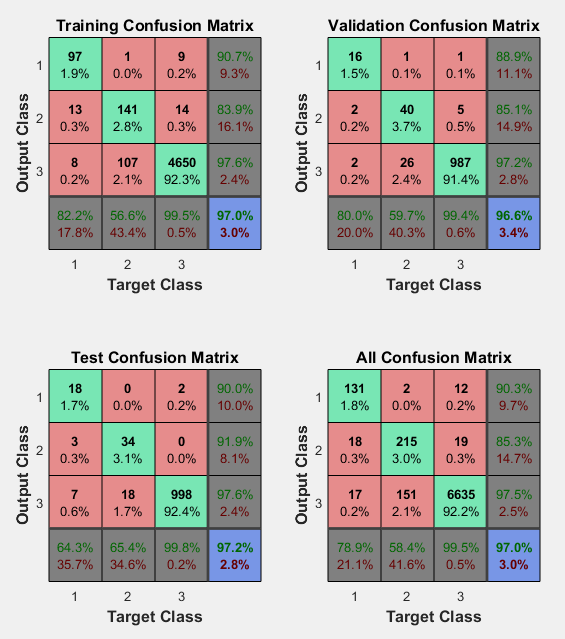
\includegraphics[width=\textwidth]{ConfMatrix.png}
	\caption{Matriz de confusión.}
\end{figure}

Al introducir datos multiplicados por 0.95 obtenemos 0.031806 de error total. Mientras que al multiplicarlos por 1.05 obtenemos 0.029306. Como vemos, se obtienen unos resultados bastante buenos.



% -------------------------------------------------------------
% Bibliography
% -------------------------------------------------------------
\newpage
\bibliography{citations}
\bibliographystyle{plainnat}

\end{document}
